\chapter{Tablas}

\begin{table}
\centering
\caption{Comparativa de estilos arquitecturales \textit{REST} y \textit{WS-*}.}
\label{restvsws}
\begin{center}
\begin{tabular}{|l|l|}\hline
\textbf{\textit{WS-*}} & \textbf{\textit{REST}} \\\hline
Cuerpo cerrado de est\'andares. & Estilo de arquitectura. \\
Orientada a la invocaci\'on remota de procedimientos. & Orientada a recursos. \\
Interfaz variable. & Interfaz uniforme.\\
Uso de HTTP opcional. & HTTP es el \'unico protocolo. \\
Descubrimiento centralizado. & Descubrimiento a trav\'es de enlaces.\\
Uso de identificadores dependientes del contexto. & Uso de identificadores globales.\\
Puede almacenar estado. & No almacena estado. \\
Permite la descripci\'on de recursos. & Los recursos son auto-descriptivos.\\\hline
\end{tabular}
\end{center}
\end{table}
\clearpage
\newpage


\begin{table}
\vspace{2.4in}
\caption{Sintaxis formal del calculo relativa al espacio de tripletes y elementos b\'asicos.}
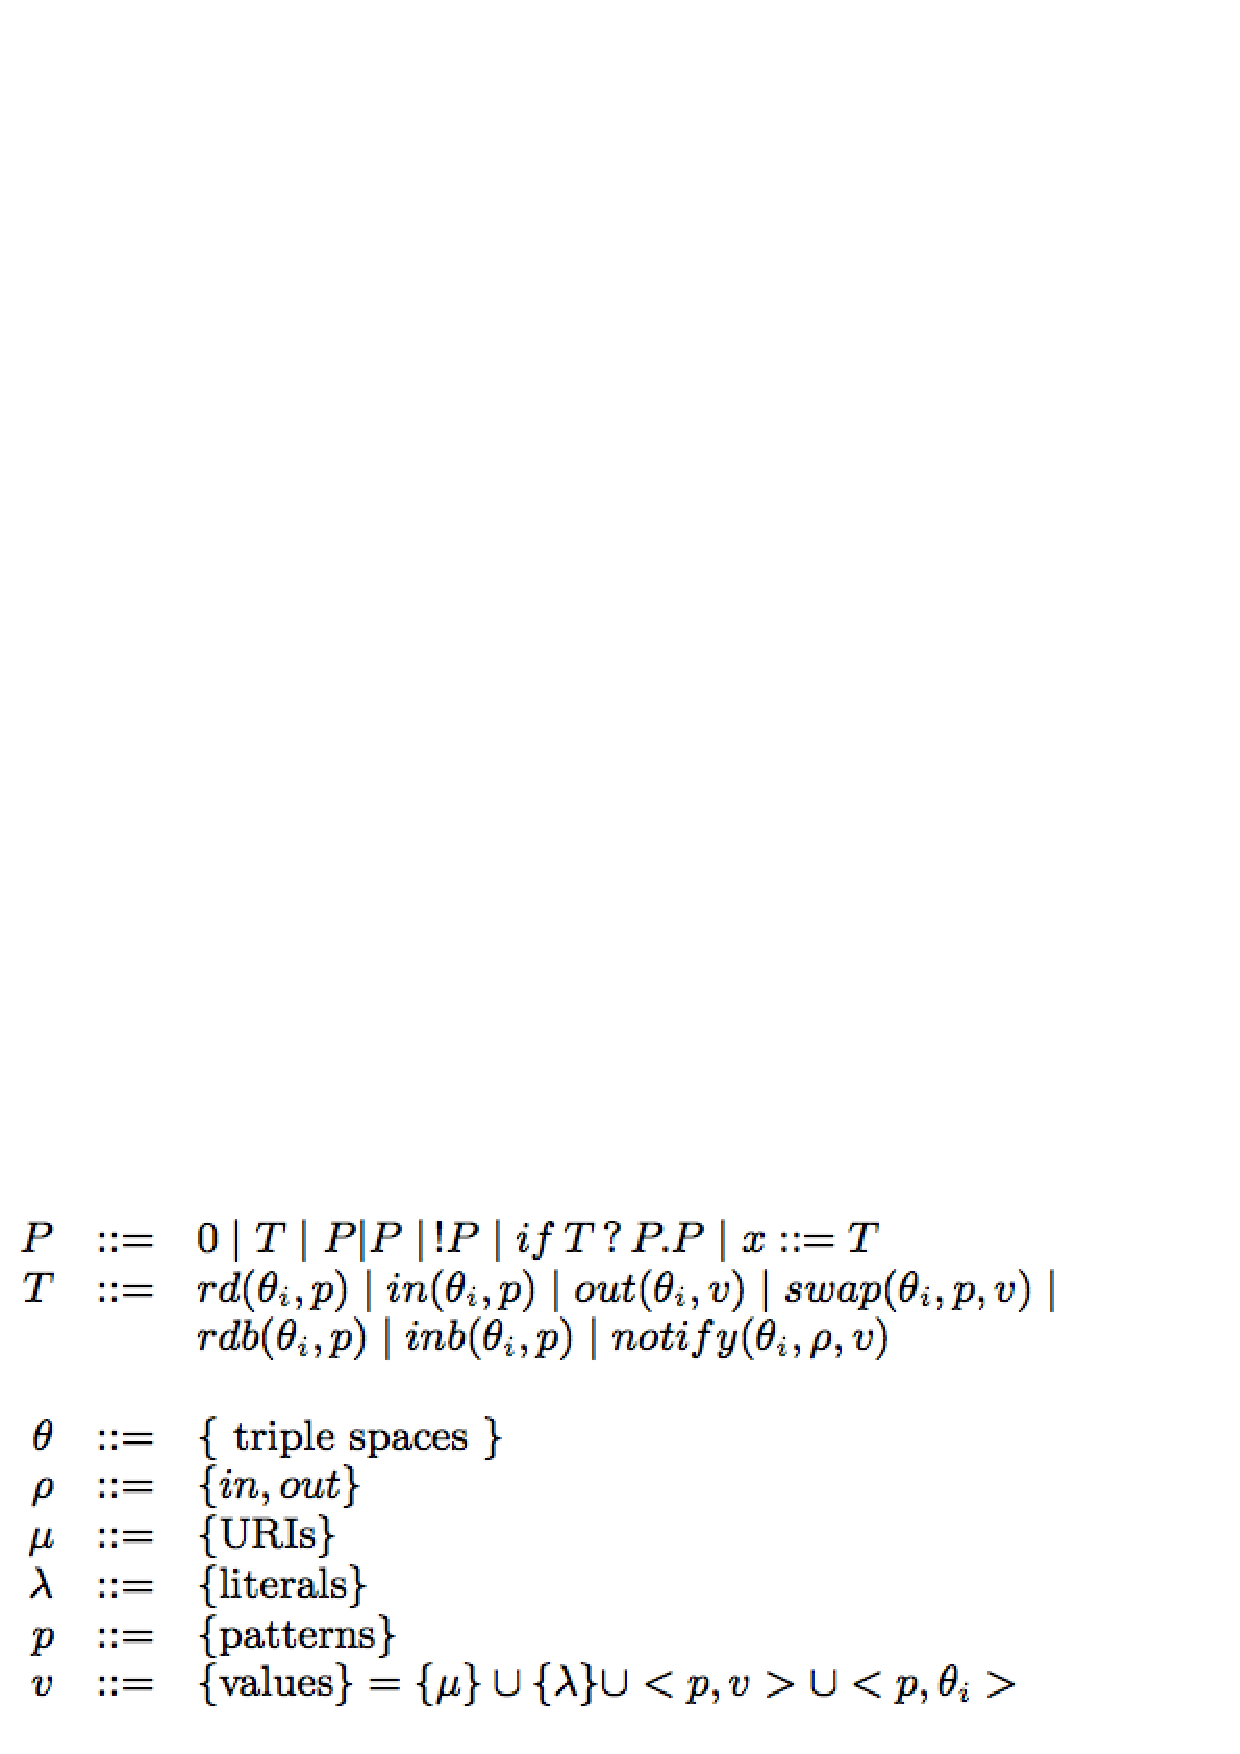
\includegraphics[width=0.8\textwidth]{tabla1}
\label{tabla1}
\end{table}

\clearpage
\newpage


\begin{table}
\vspace{2.4in}
\caption{Sem\'antica operacional del calculo relativa al espacio de tripletes y operaciones b\'asicas.}
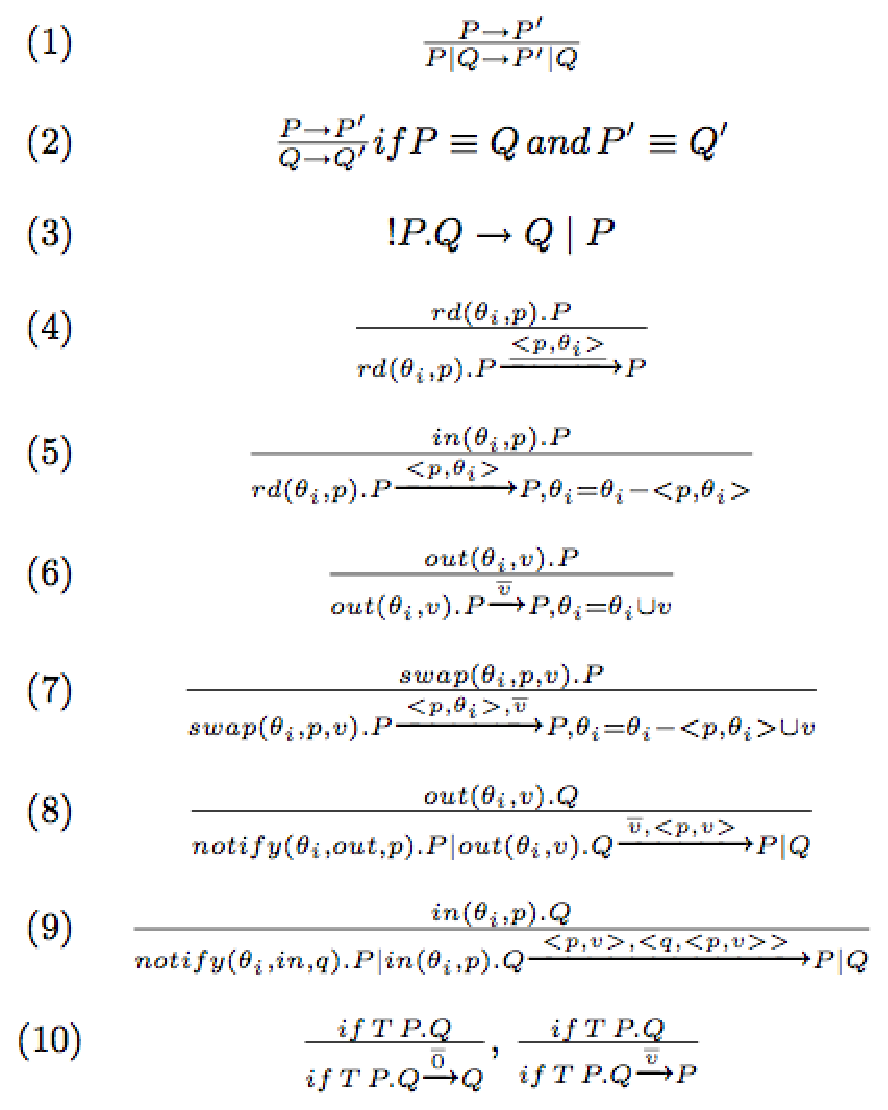
\includegraphics[width=0.8\textwidth]{tabla2}
\label{tabla2}
\end{table}
\clearpage
\newpage

\begin{table}
\vspace{2.4in}
\caption{Sem\'antica operacional del c\'alculo relativa a la comunicaci\'on entre procesos.}
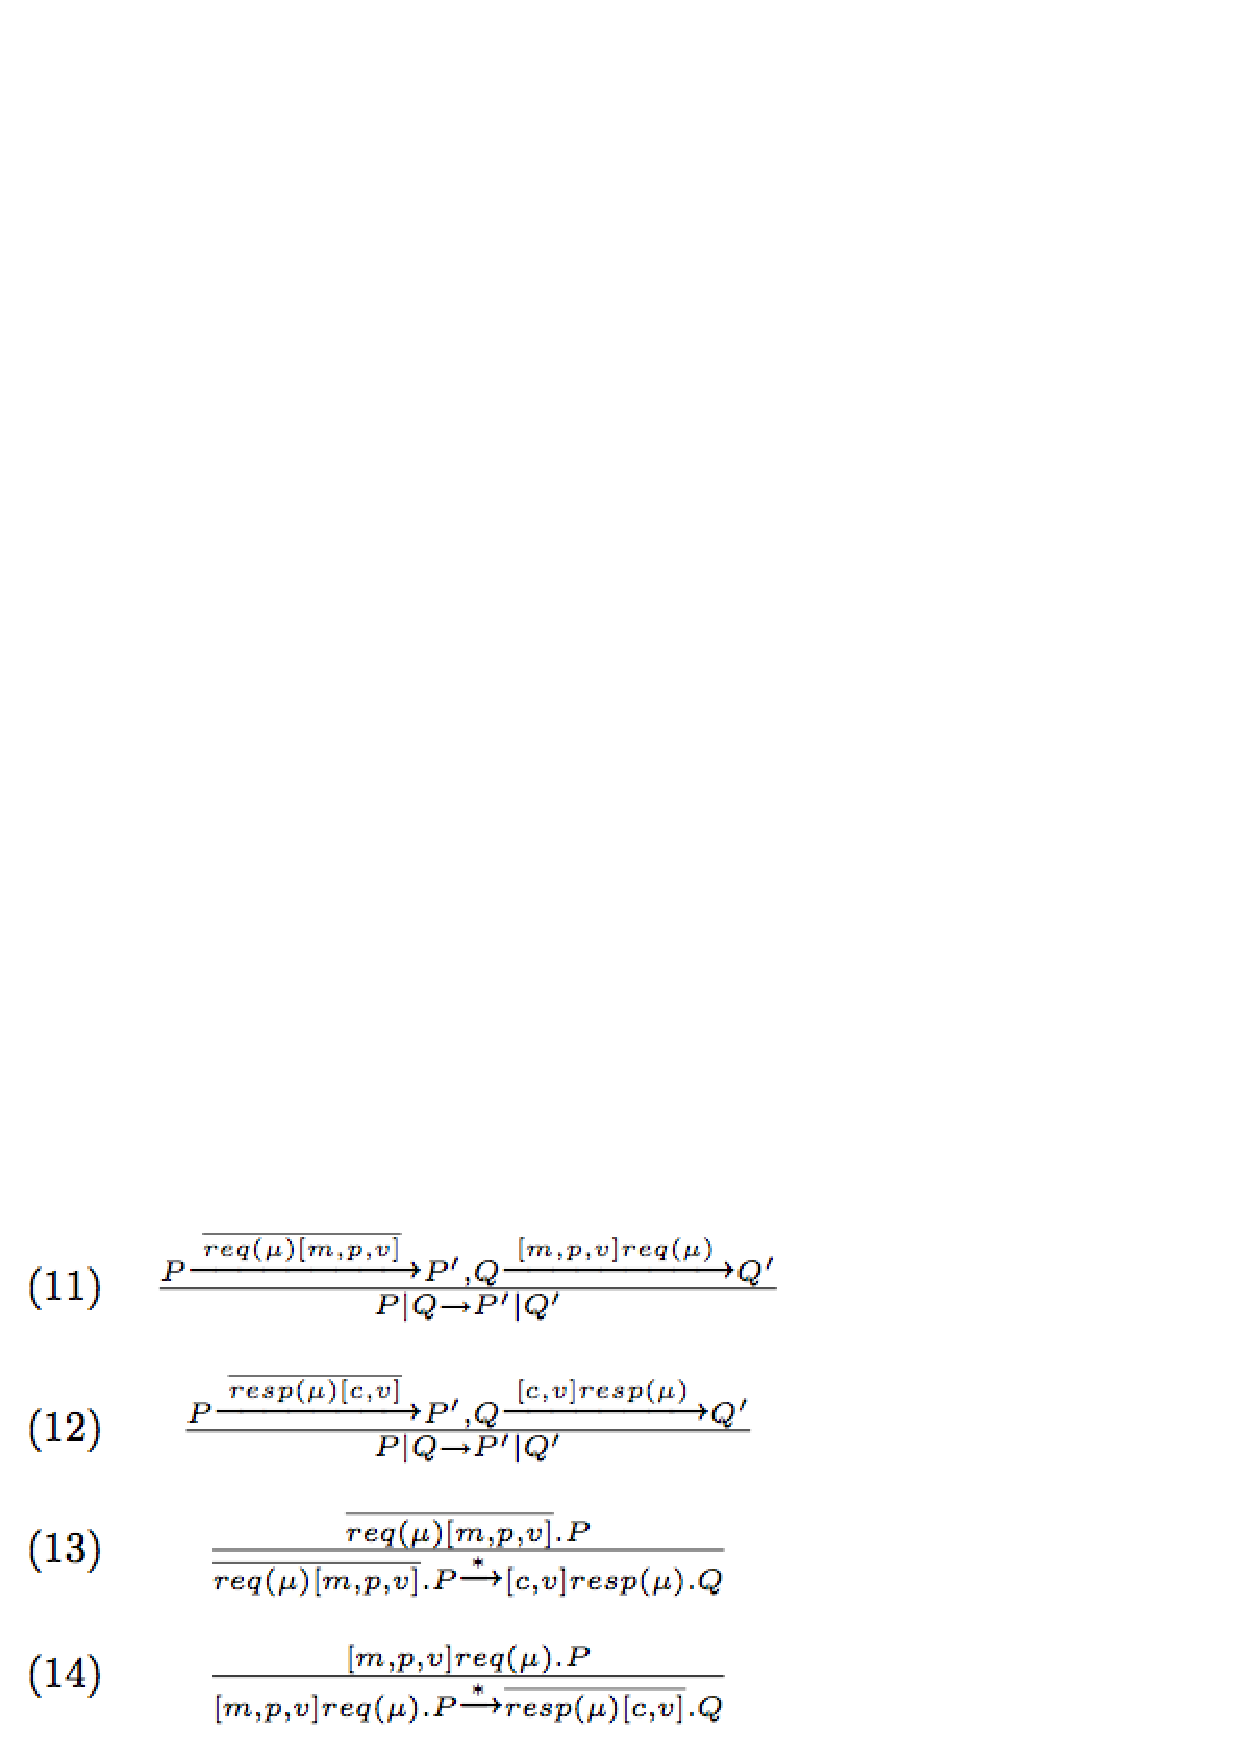
\includegraphics[width=0.8\textwidth]{tabla3}
\label{tabla3}
\end{table}
\clearpage
\newpage

\begin{table}
\vspace{2.4in}
\caption{Descripci\'on param\'etrica de un recurso \textit{REST} sem\'antico simple.}
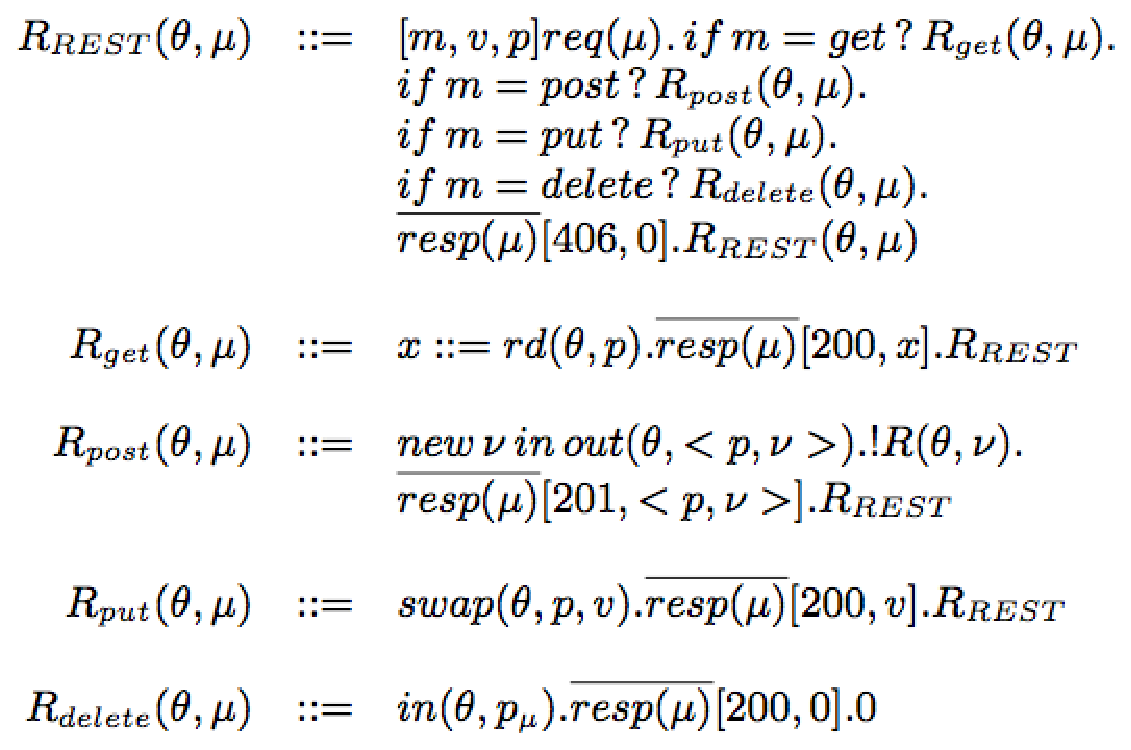
\includegraphics[width=0.8\textwidth]{tabla4}
\label{tabla4}
\end{table}
\clearpage
\newpage

\begin{table}
\vspace{2.4in}
\caption{Descripci\'on \textit{RDF} de un servicio \textit{REST} sem\'antico.}
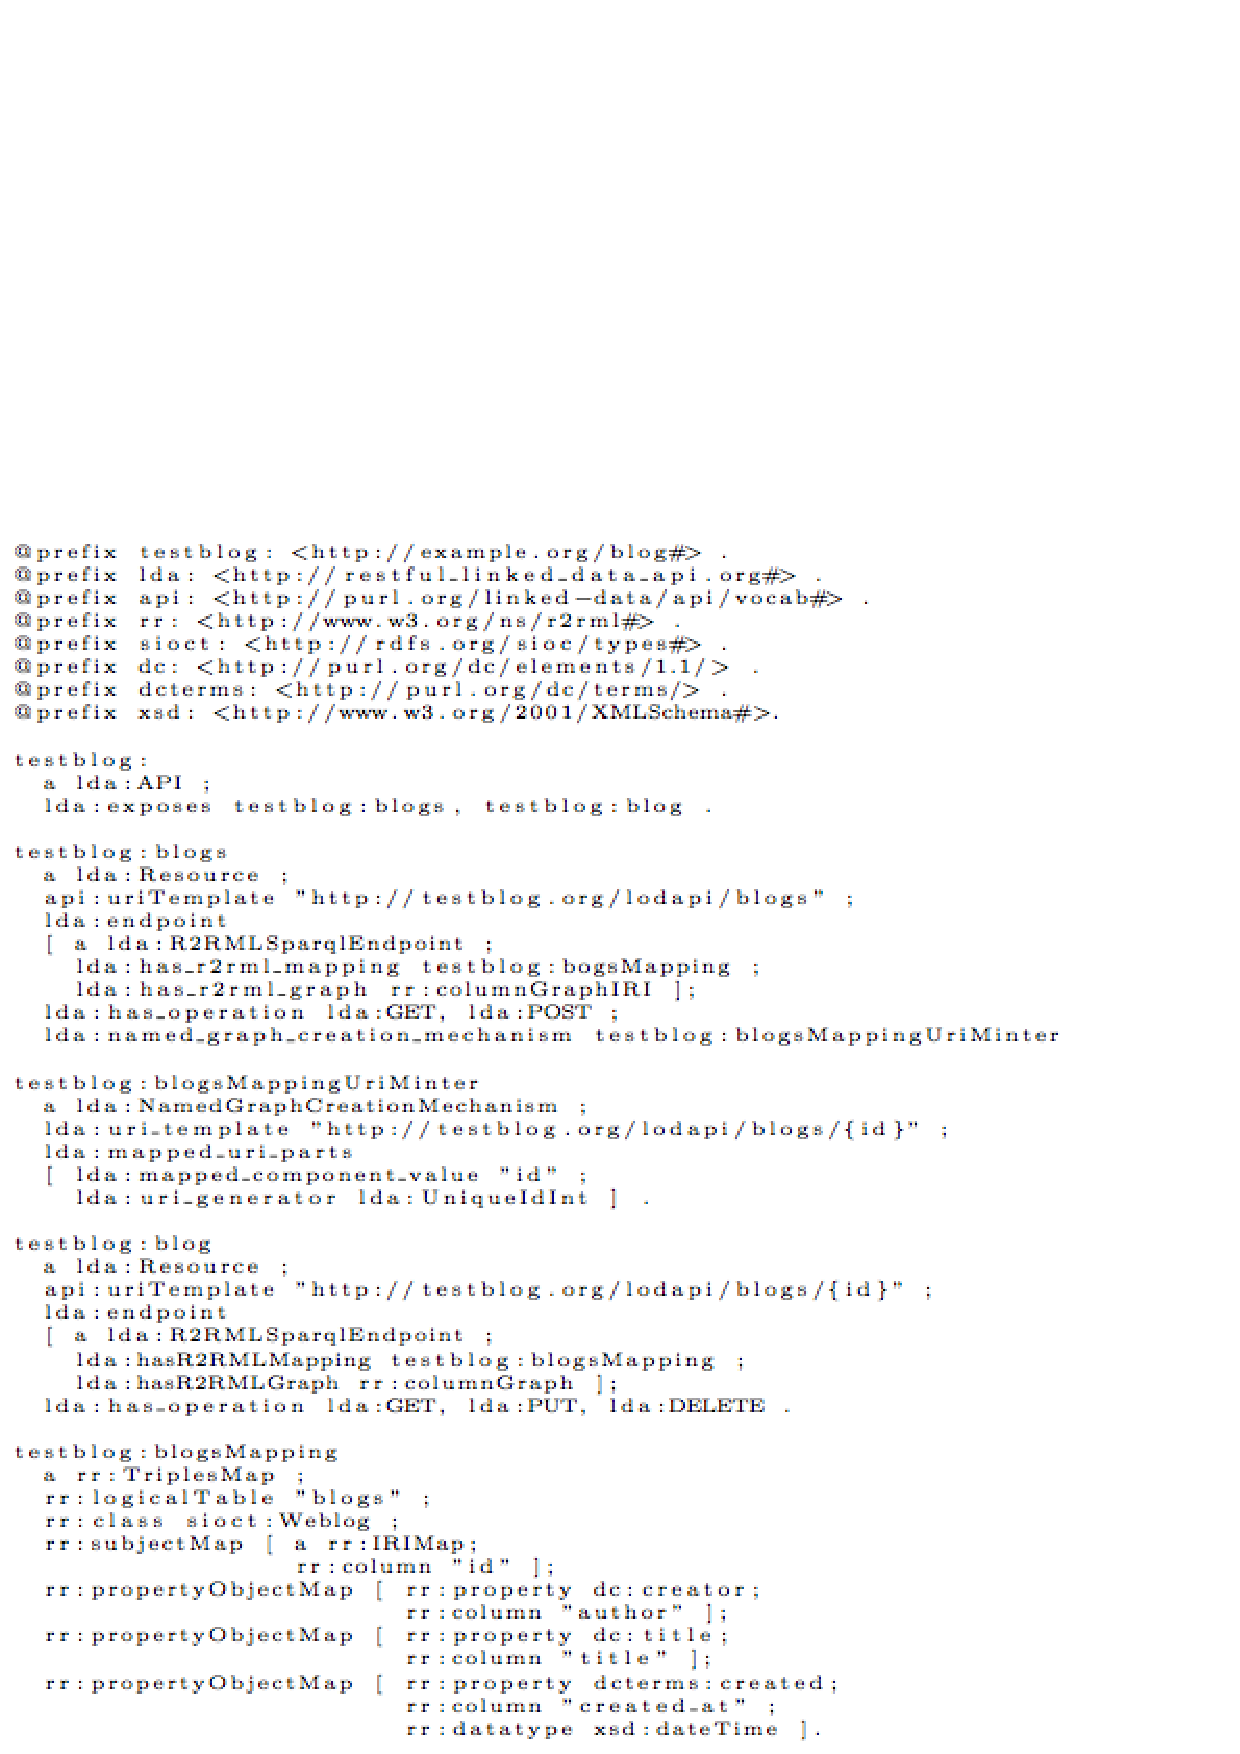
\includegraphics[width=0.8\textwidth]{tabla5}
\label{tabla5}
\end{table}
\clearpage
\newpage

\begin{table}
\vspace{2.4in}
\caption{Consulta \textit{SPARQL} para una peticion \textit{HTTP} \textit{GET}.}
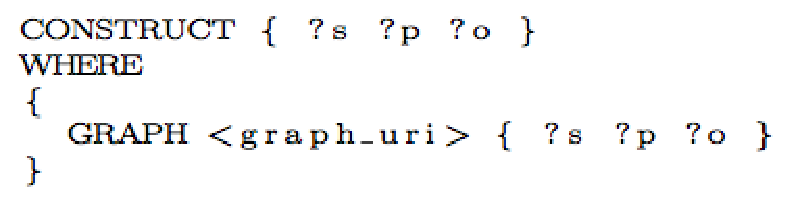
\includegraphics[width=0.8\textwidth]{tabla6}
\label{tabla6}
\end{table}
\clearpage
\newpage

\begin{table}
\vspace{2.4in}
\caption{Consulta \textit{SPARQL} para una petici\'on \textit{HTTP} \textit{POST}.}
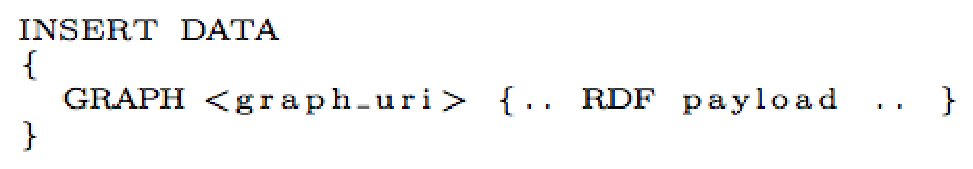
\includegraphics[width=0.8\textwidth]{tabla7}
\label{tabla7}
\end{table}
\clearpage
\newpage


\begin{table}
\centering
\caption{\textit{Grafos con nombre} frente a recursos \textit{RDF}.}
\label{named_graph_vs_resource_uri}
\begin{center}
\begin{tabular}{|l|l|}\hline
\textbf{\textit{Grafo con nombre}} & \textbf{\textit{Recurso RDF}} \\\hline
Identificado por un \textit{URI}. & Identificado por un \textit{URI}. \\
Recurso de informaci\'on. & No recurso de informaci\'on.\\
Identifica el \textit{grafo con nombre}. & Aparece dentro del \textit{grafo con nombre}.\\
Desreferenciable usando \textit{HTTP} & No desreferenciable usando \textit{HTTP}\\\hline
\end{tabular}
\end{center}
\end{table}
\clearpage
\newpage


\begin{table}
\vspace{2.4in}
\caption{Consulta \textit{SPARQL} para una petici\'on \textit{HTTP} \textit{PUT}.}
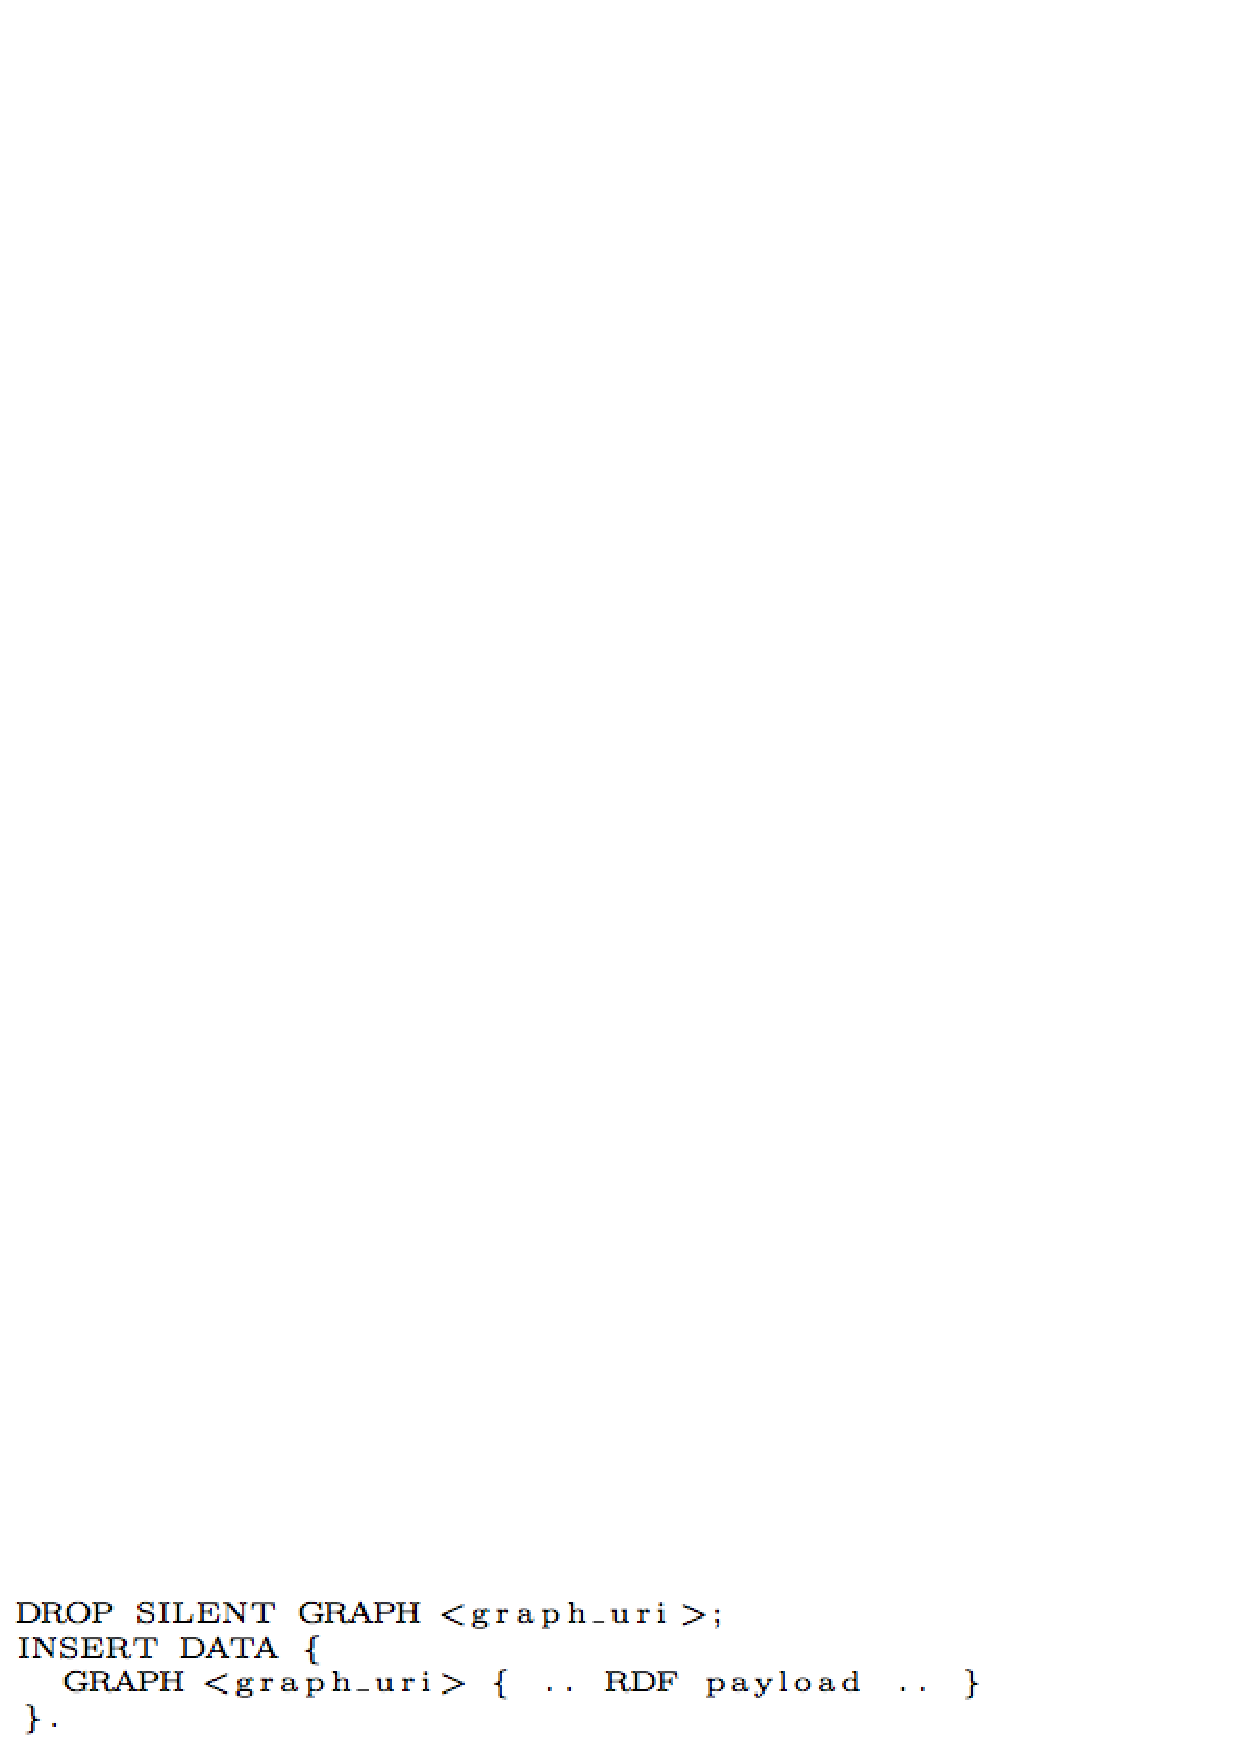
\includegraphics[width=0.8\textwidth]{tabla8}
\label{tabla8}
\end{table}
\clearpage
\newpage


\begin{table}
\vspace{2.4in}
\caption{Consulta \textit{SPARQL} para una petici\'on \textit{HTTP} \textit{DELETE}.}
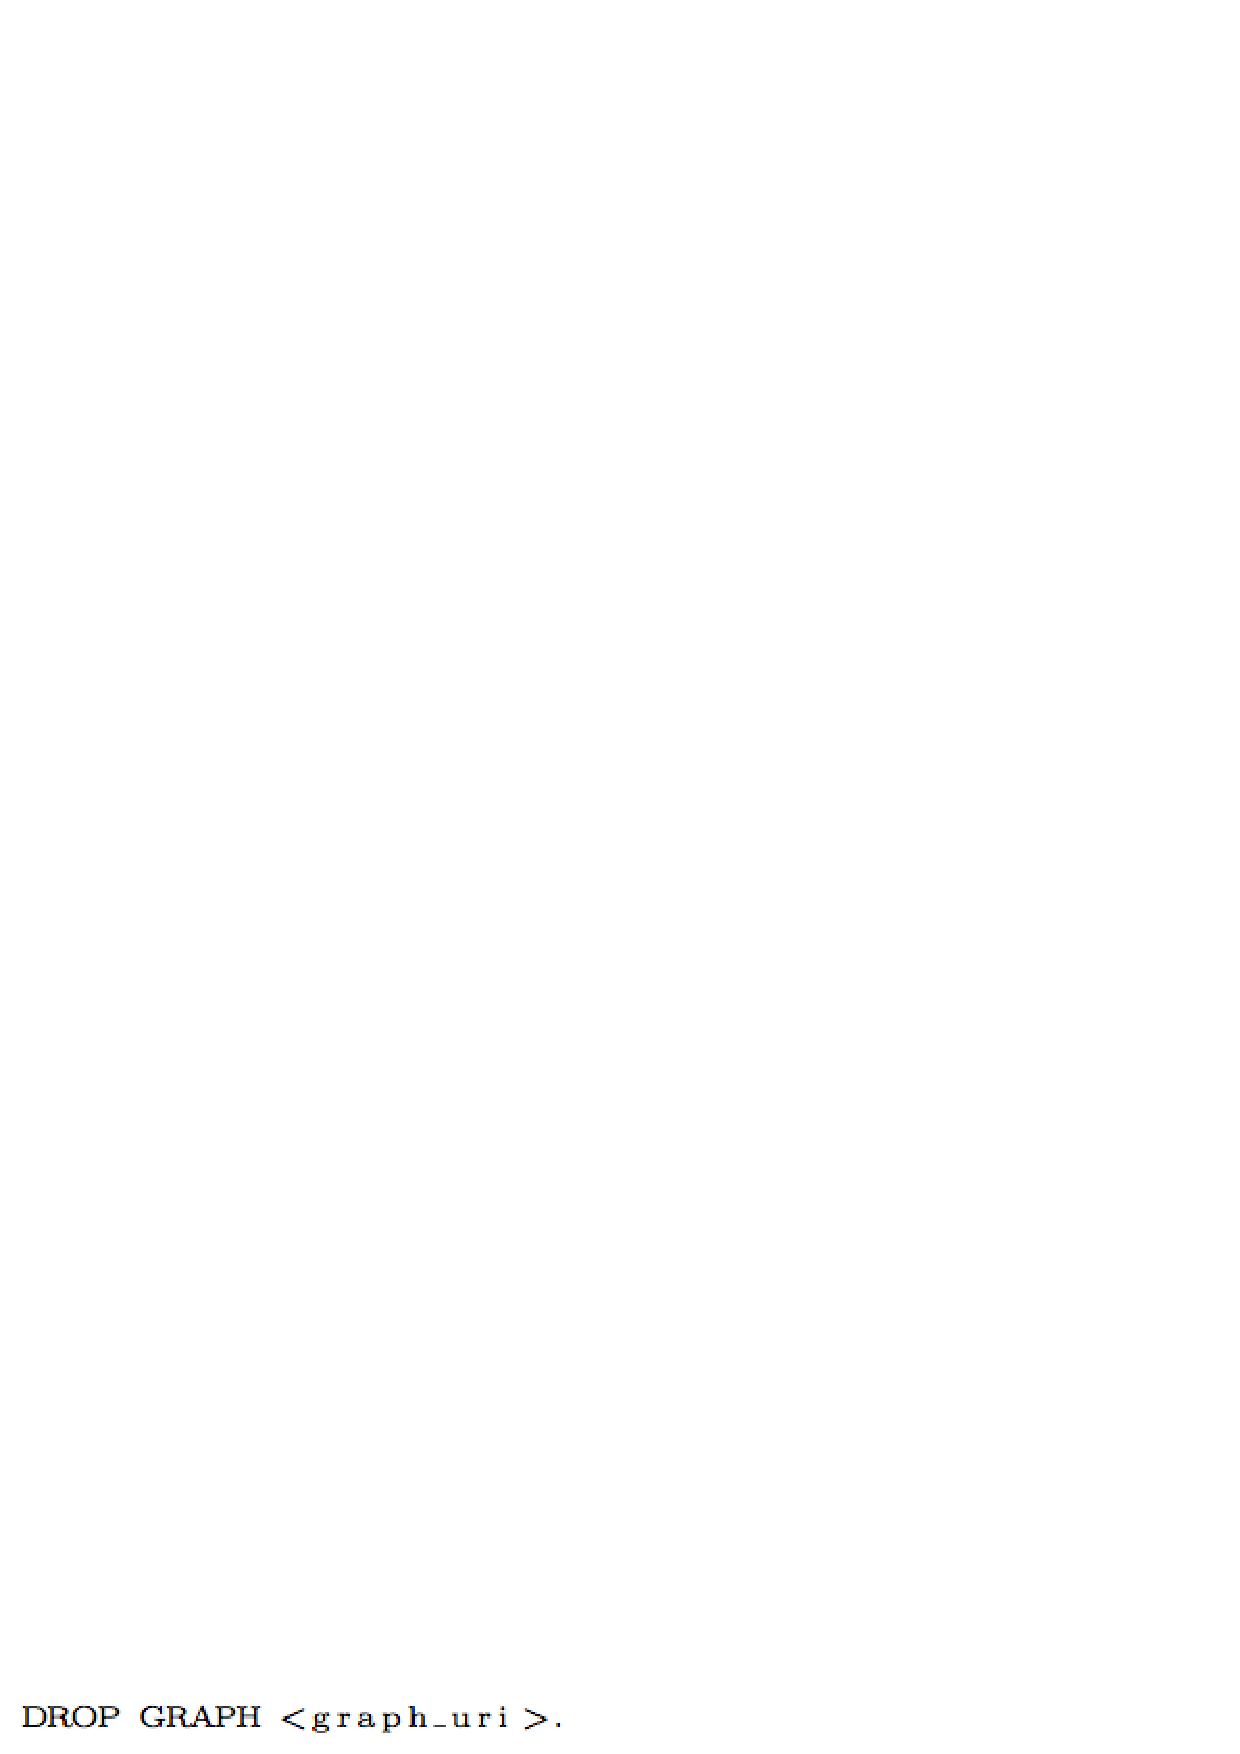
\includegraphics[width=0.8\textwidth]{tabla9}
\label{tabla9}
\end{table}
\clearpage
\newpage


\begin{table}
\vspace{2.4in}
\caption{Sintaxis \textit{EBNF} de \textit{R2RML}.}
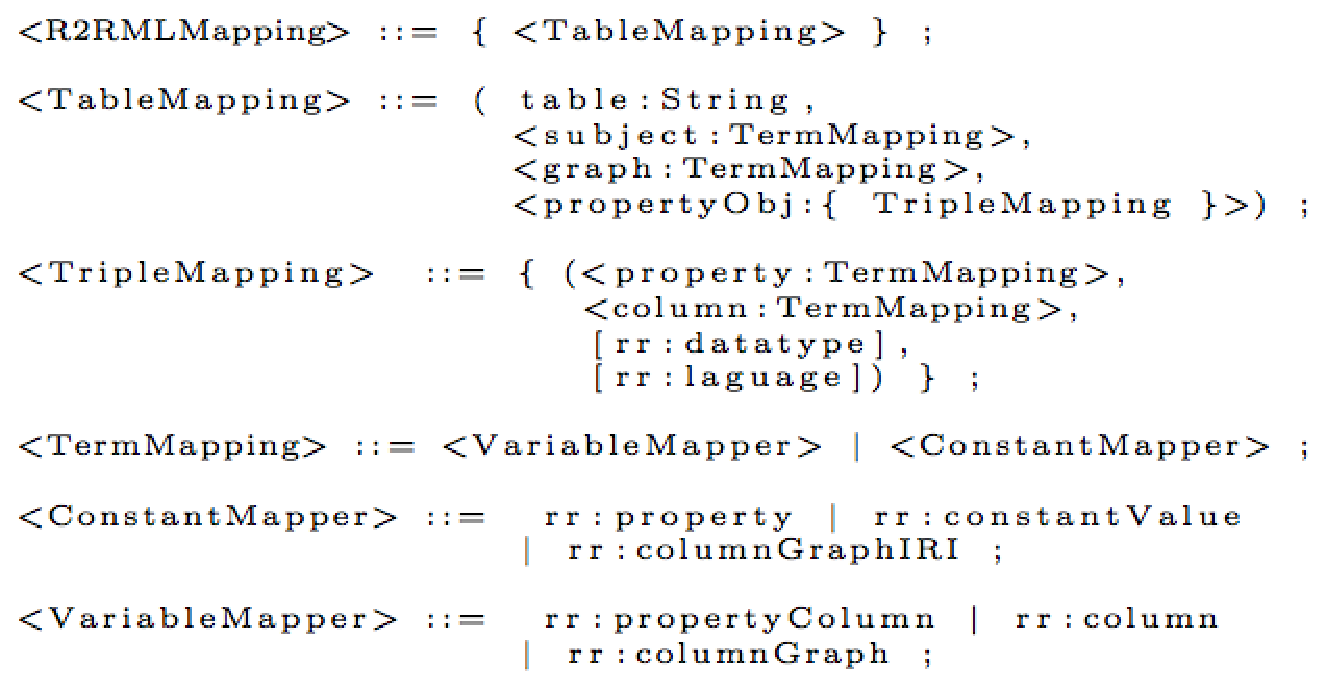
\includegraphics[width=0.8\textwidth]{tabla10}
\label{tabla10}
\end{table}
\clearpage
\newpage


\begin{table}
\vspace{2.4in}
\caption{Sintaxis de los \textit{QuadPatterns}.}
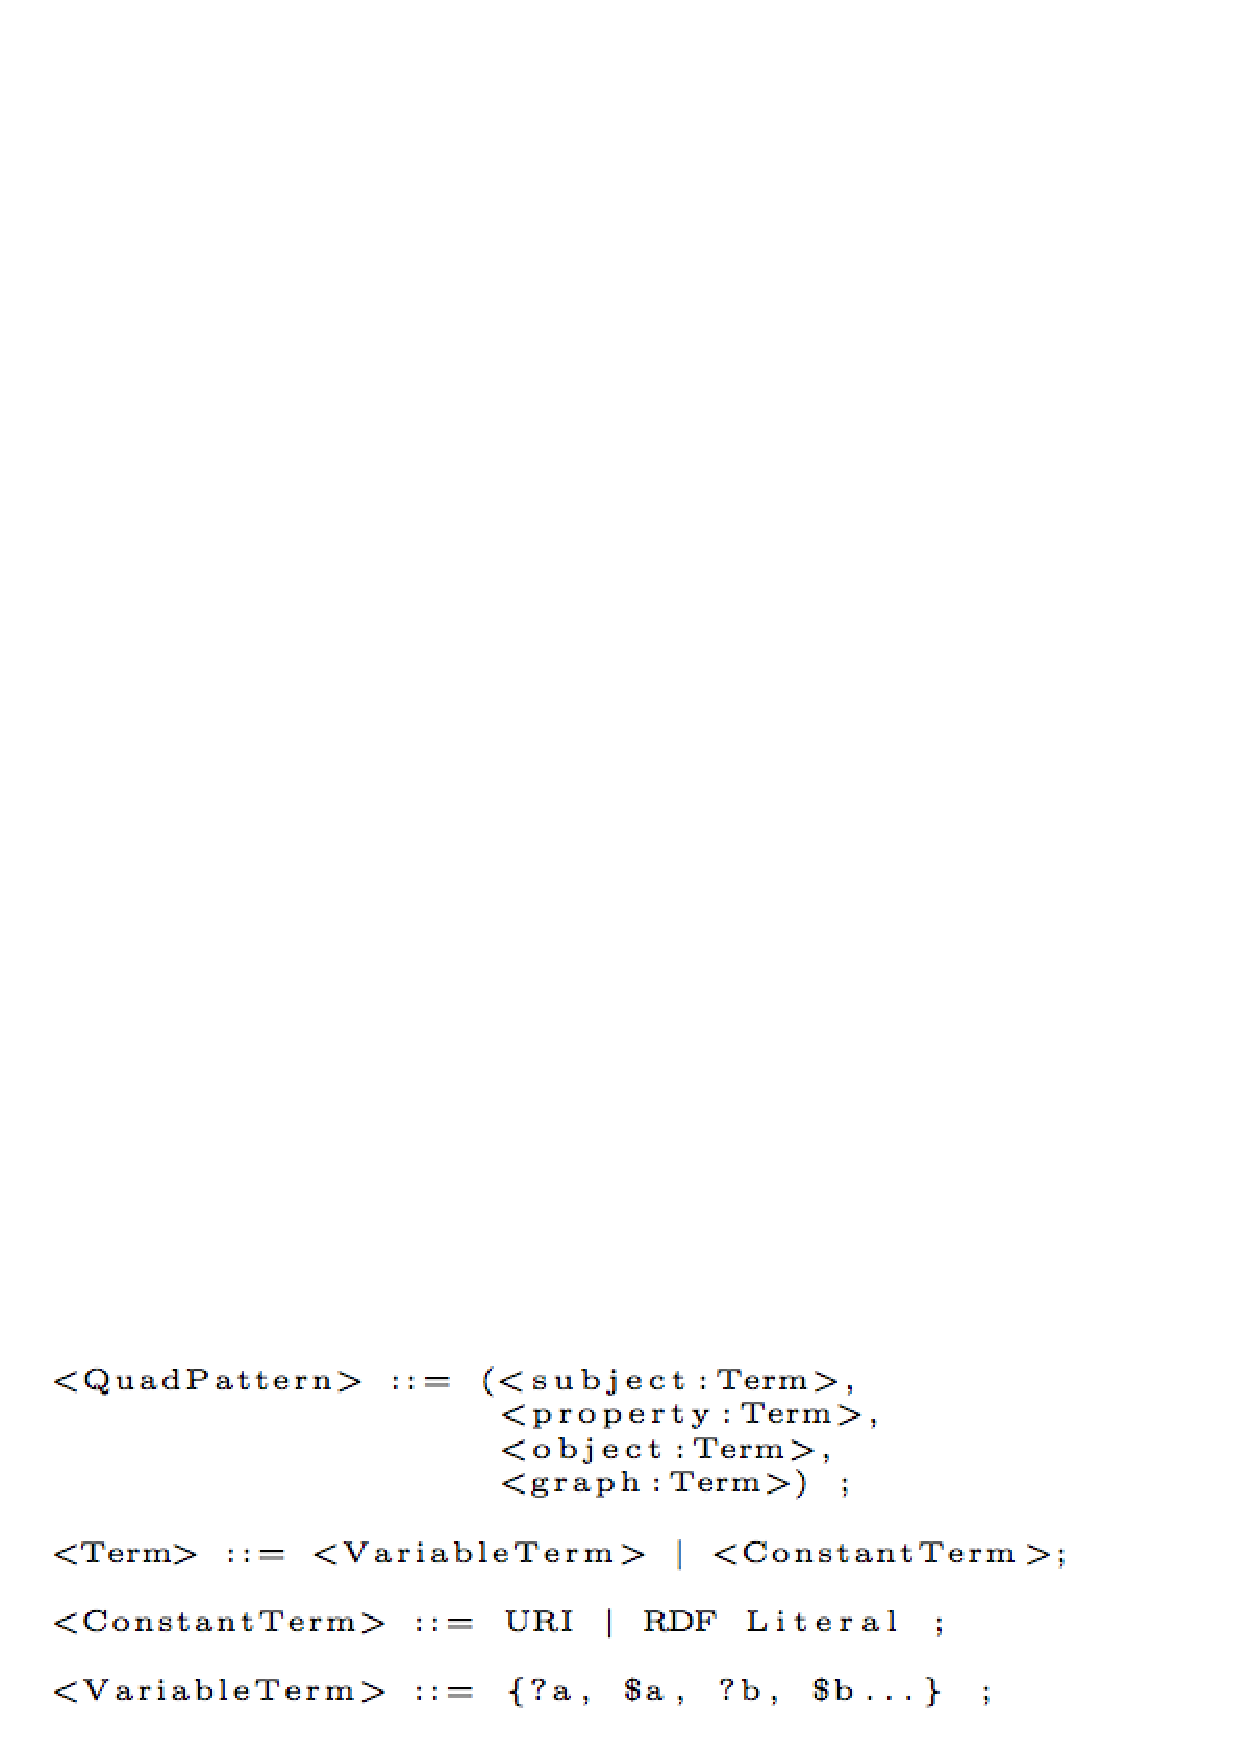
\includegraphics[width=0.8\textwidth]{tabla11}
\label{tabla11}
\end{table}
\clearpage
\newpage


\begin{table}
\vspace{2.4in}
\caption{Algoritmo 1: Construcci\'on de \textit{QuadMatcher} para una tranformaci\'on \textit{R2RML}.}
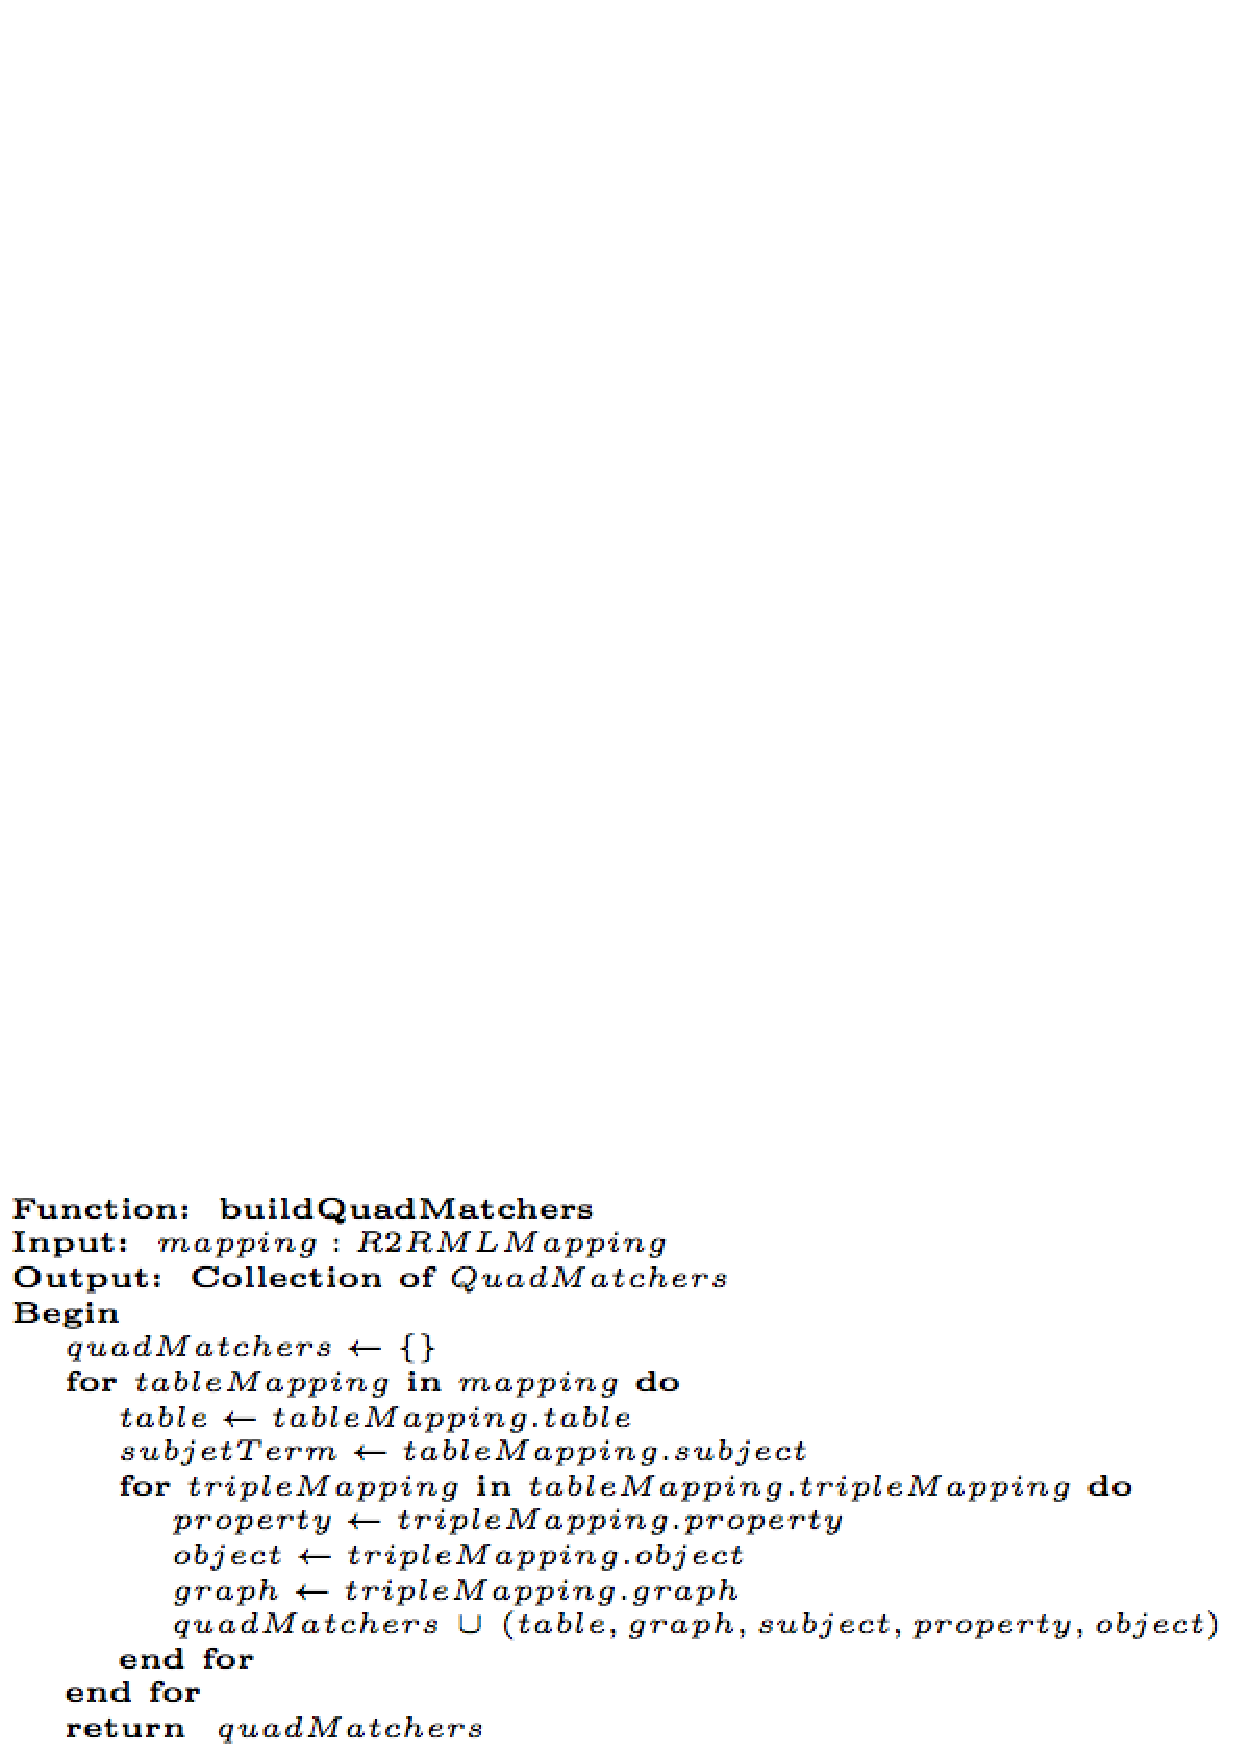
\includegraphics[width=0.8\textwidth]{algoritmo1}
\label{alg1}
\end{table}
\clearpage
\newpage


\begin{table}
\vspace{2.4in}
\caption{Algoritmo 2: Procedimiento para comprobar si un \textit{QuadPattern} y un \textit{QuadMatcher} son compatibles.}
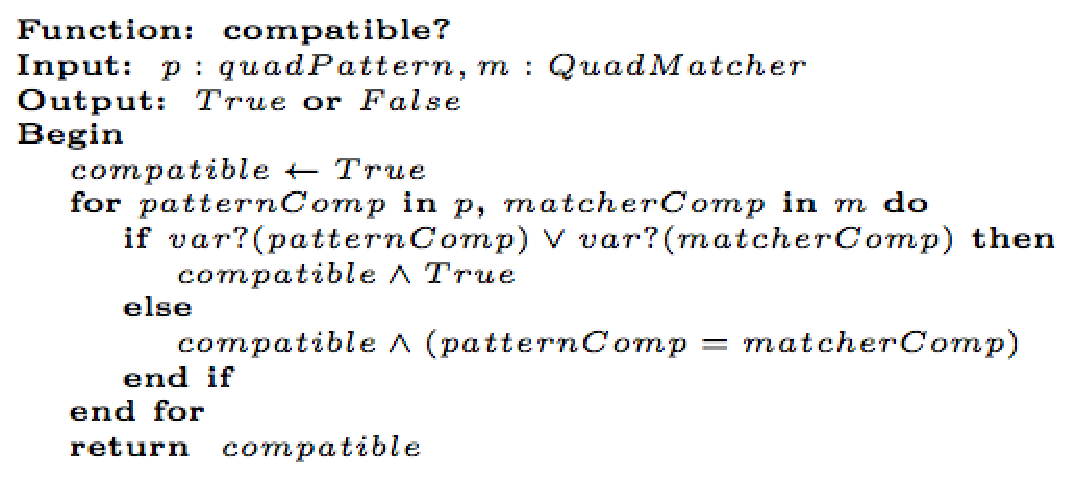
\includegraphics[width=0.8\textwidth]{algoritmo2}
\label{alg2}
\end{table}
\clearpage
\newpage

\begin{table}
\vspace{2.4in}
\caption{Algoritmo 3: Composici\'on de una consulta \textit{SELECT} para un \textit{QuadPattern} y un conjunto de \textit{QuadMatchers}.}
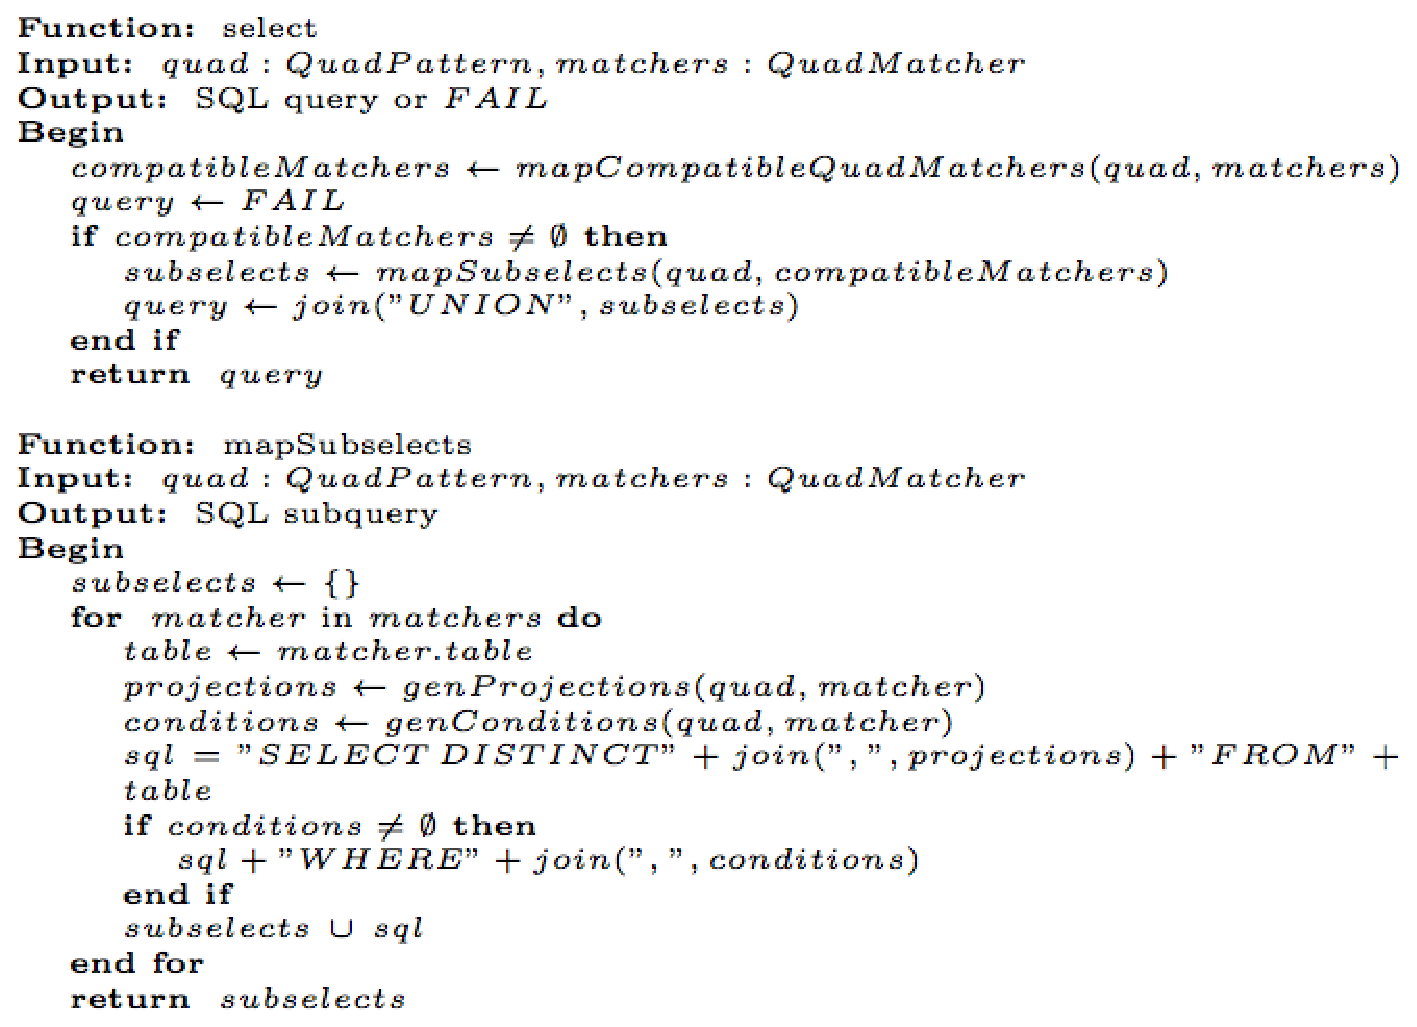
\includegraphics[width=0.8\textwidth]{algoritmo3}
\label{alg3}
\end{table}
\clearpage
\newpage

\begin{table}
\vspace{2.4in}
\caption{Algoritmo 4: Inserci\'on de un \textit{QuadPattern} para un conjunto de \textit{QuadMatchers}.}
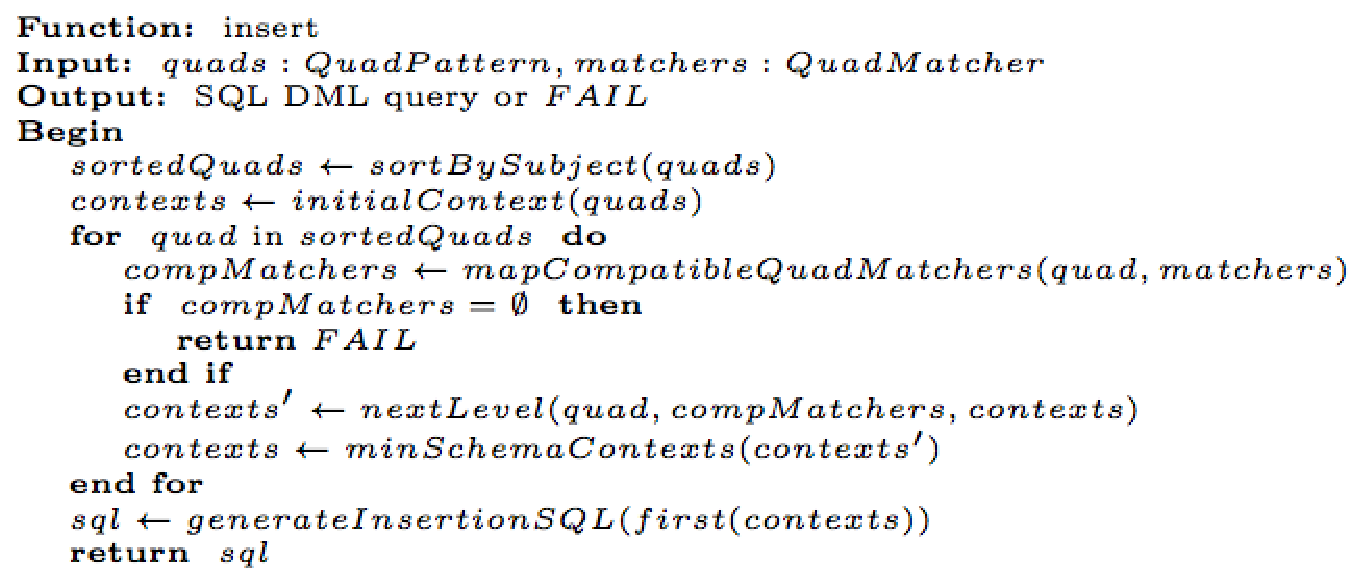
\includegraphics[width=0.8\textwidth]{algoritmo4}
\label{alg4}
\end{table}
\clearpage
\newpage


\begin{table}
\vspace{2.4in}
\caption{Algoritmo 5: M\'etrica de coste.}
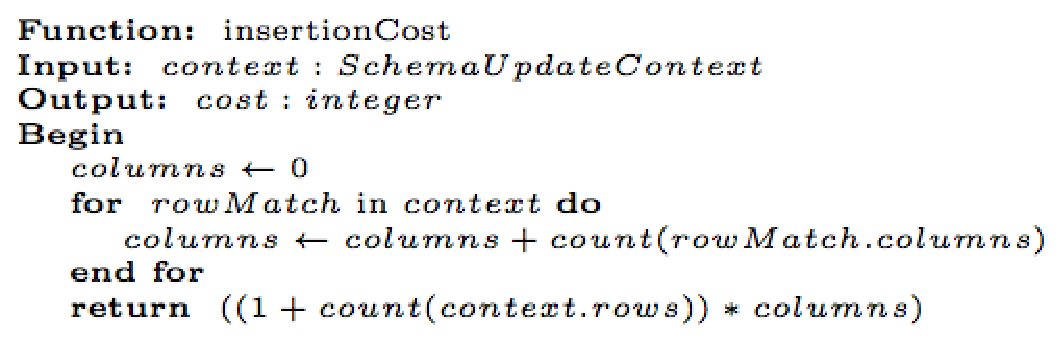
\includegraphics[width=0.8\textwidth]{algoritmo5}
\label{alg5}
\end{table}
\clearpage
\newpage

\begin{table}
\vspace{2.4in}
\caption{Algoritmo 6: Composici\'on de una consulta para eliminar un \textit{QuadPattern} para un conjunto de \textit{QuadMatchers}.}
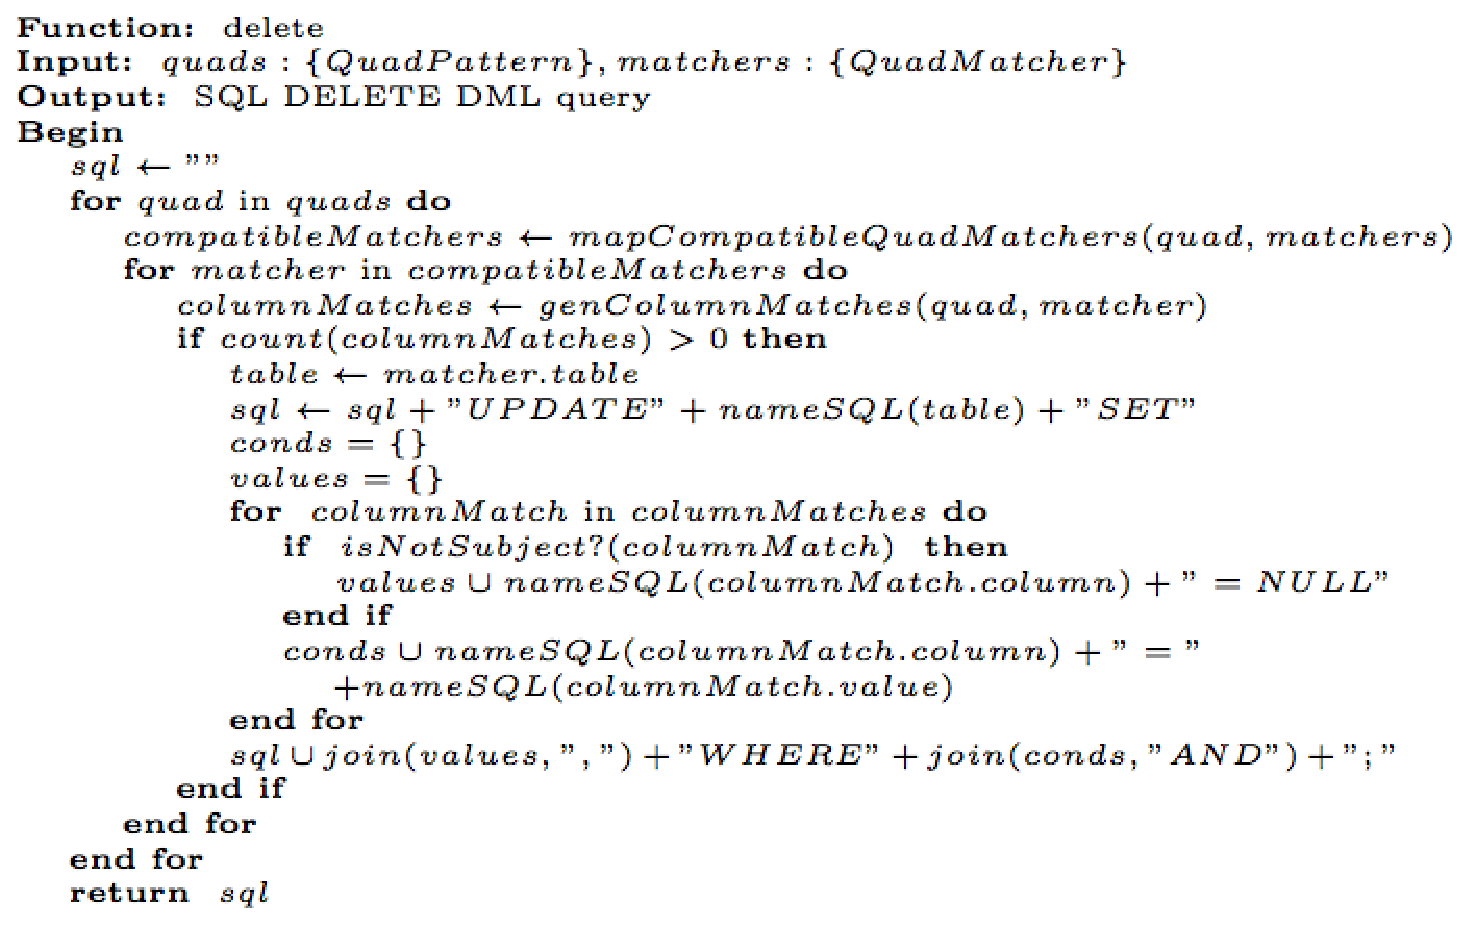
\includegraphics[width=0.8\textwidth]{algoritmo6}
\label{alg6}
\end{table}
\clearpage
\newpage


\begin{table}
\vspace{2.4in}
\caption{Pruebas de rendimiento \textit{LUBM} para el repositorio \textit{RDF}}
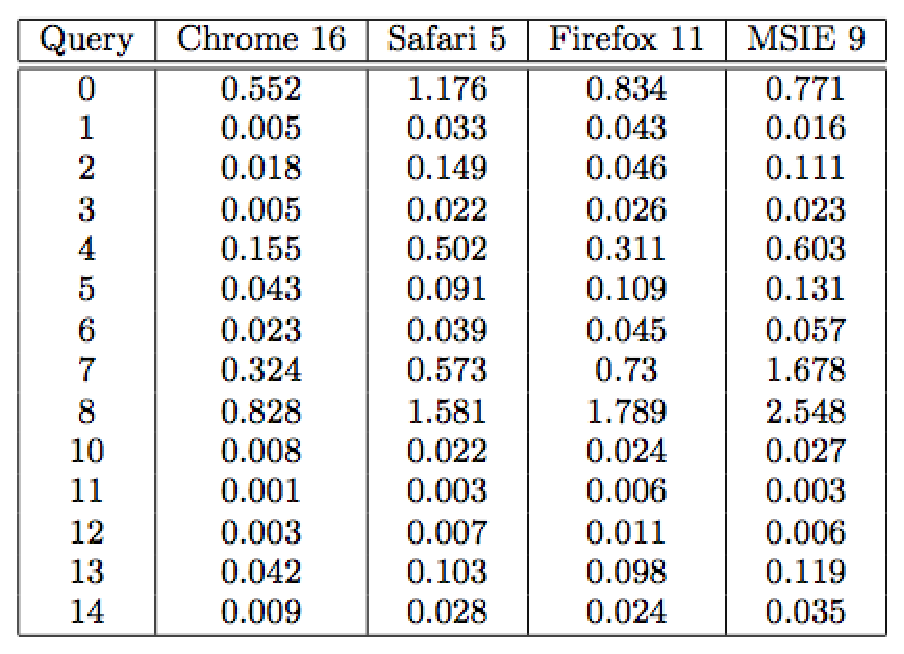
\includegraphics[width=0.8\textwidth]{tabla12}
\label{tabla12}
\end{table}
\clearpage
\newpage


\begin{table}
\vspace{2.4in}
\caption{Definici\'on de una visualizaci\'on usando la gram\'atica de gr\'aficos.}
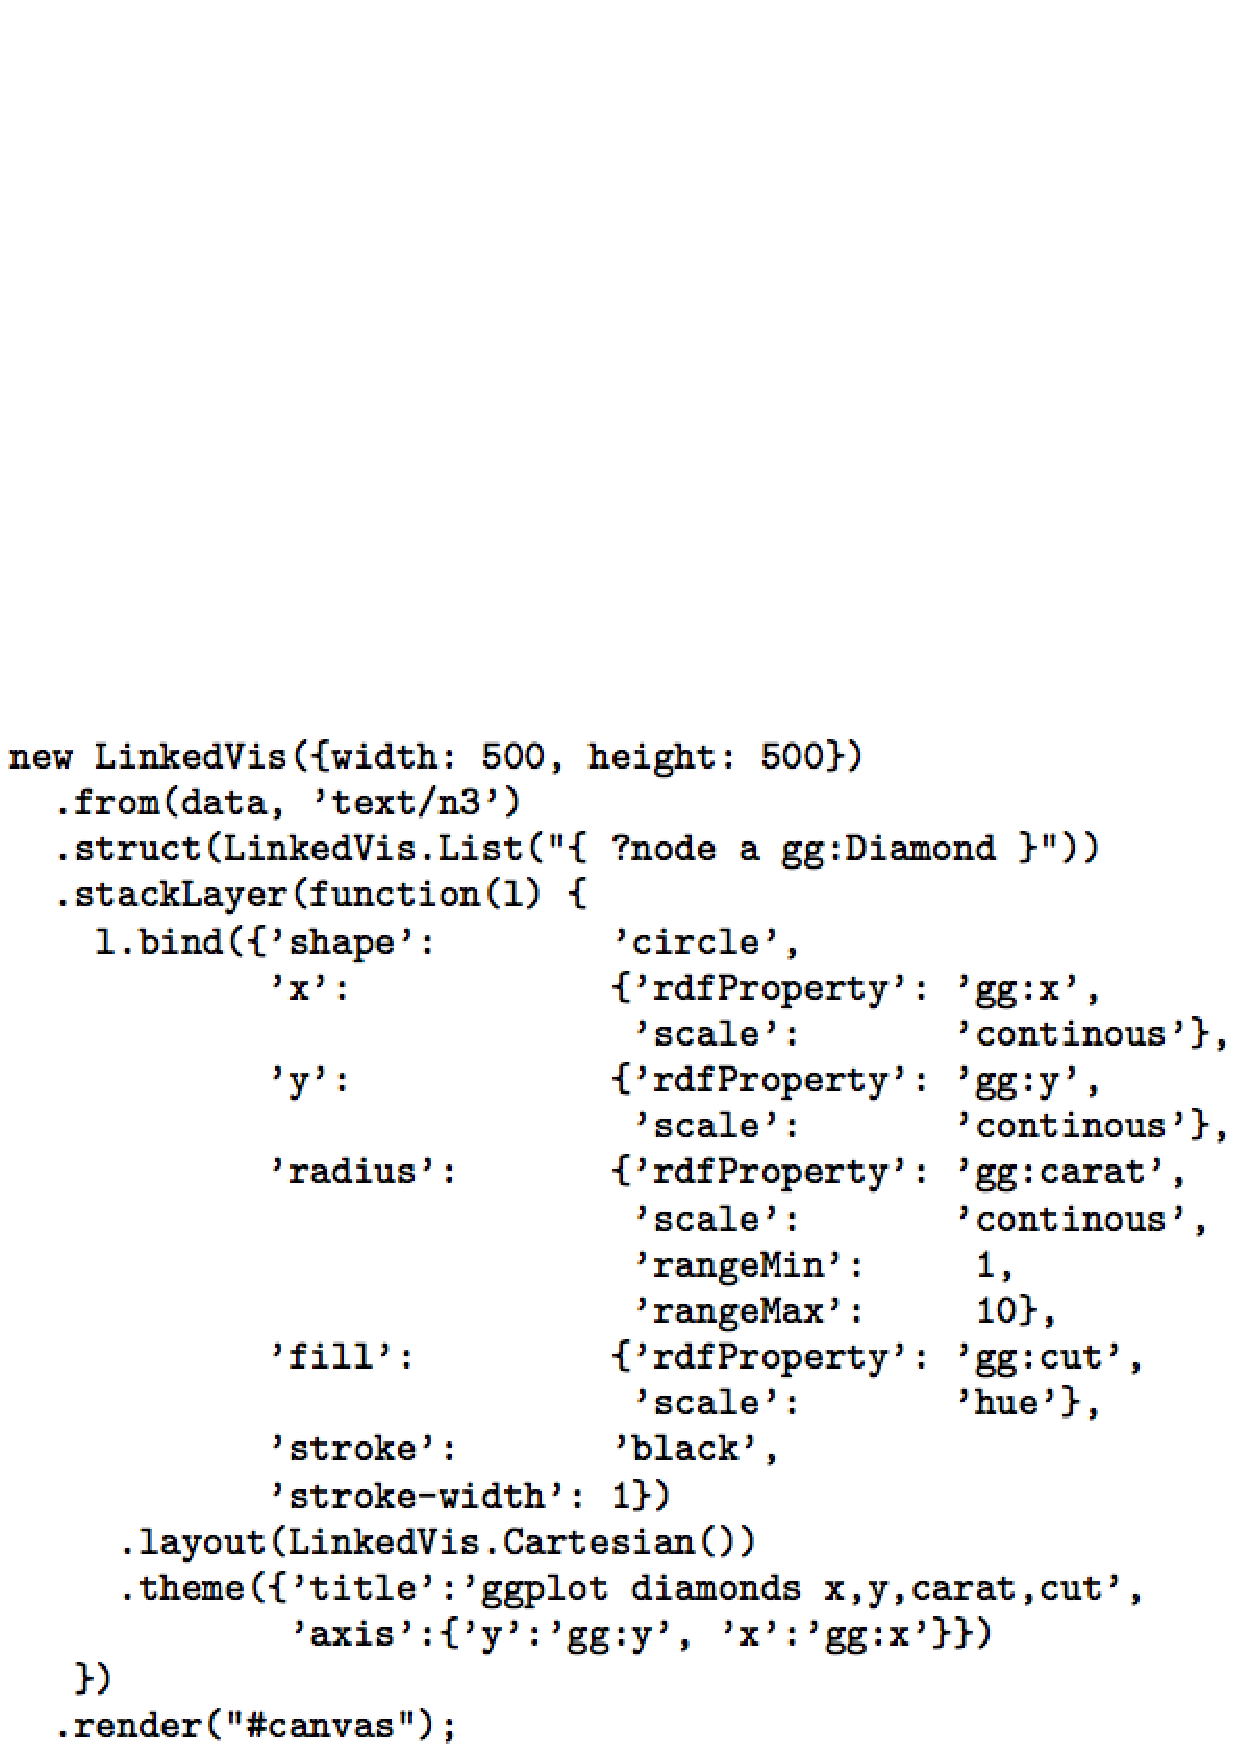
\includegraphics[width=0.8\textwidth]{tabla13}
\label{tabla13}
\end{table}
\clearpage
\newpage


